En este apartado nos centramos en corroborar que los pasos de la implementaci\'on se dieron acorde a lo que cada m\'etodo visto propone. Para ello, creamos dos instancias en la cual se podr\'an visualizar con facilidad los cambios generados al aplicar el efecto de slowmotion. De hecho, uno de ellos se basar\'a de reproducir una sola im\'agen durante todo el video. El restante se basar\'a en observar el cambio entre los dos extremos que proporciona la escala de grises, es decir, de negro a blanco.
%---------------------------------------------------------------
\subsubsection{Negro a blanco}

Nos situamos primero en el caso donde el video se compone de dos tipos de frames, repetidos una cierta cantidad de veces. La particularidad de dichos frames es que son completamente uniformes: vistos como matrices, todos sus elementos son iguales. Debido a que estamos trabajando sobre escala de grises, decidimos clasificar al tipo $A$ como un frame con todos sus p\'ixeles en negro (equivalente a $0$) y el tipo $B$ con p\'ixeles en blanco (equivalente a $255$).

Haber escogido dos valores que representan los extremos en la escala de representaci\'on nos da una mejor intuici\'on del resultado esperado. Con esto nos adelantamos a decir que el video ralentizado mostrará una trancisión de $A$ a $B$ pasando por los diferentes tonos de gris.

\subsubsection*{\bf{Vecino m\'as cercano}}

Sabemos que su idea reside en crear los cuadros intermedios copiando de un extremo u otro, tal como se explic\'o durante el desarrollo. Por ende, el resultado que \'este dar\'a al aplicarlo sobre el video ser\'a bastante trivial. De hecho lo \'unico que se podr\'a apreciar es la mayor duraci\'on del video resultante con respecto al original.

\subsubsection*{Resultado}

Comprobamos que al mirar los frames intermedios como matrices, estos se igualaron con su frame original m\'as cercano. Si al par\'ametro de cantidad de frames a adherir se le asigna un n\'umero impar, en teor\'ia el valor del extremo derecho (en este caso, el blanco) tendr\'ia mayor presencia. Sin embargo, como la diferencia es de un solo frame adicional, no se nota visualmente en la pr\'actica debido a la cantidad de frames por segundo a la que se reproduce el video (24 fps, con lo cual el blanco aparece $\frac{1}{24}s$ más, imperceptible para el ojo humano).

\subsubsection*{\bf{Interpolaci\'on lineal}}

Nos inclinamos a una perspectiva que abarca mayor seriedad, ya que su comprobaci\'on se justificar\'a por una evaluación matem\'atica. Si los únicos dos puntos a trazar son el $(x_0,y_0) = (0,0)$ y $(x_1,y_1) = (1,255)$, luego la funci\'on a considerar tendr\'a la forma:

$$f(x) = y_0 + (y_1-y_0) * \frac{x - x_0}{x_1 - x_0} = 255 * \frac{x}{255} = x$$

Con esto \'ultimo, se puede considerar que tampoco traer\'a mucha dificultad al momento de analizar correctitud.

\subsubsection*{Resultado}

Fuimos elevando el par\'ametro de entrada, agregando m\'as frames de por medio. De esta manera, el m\'etodo se encargaba de evaluar cada $f(x) = x$, con $x \in \{ \frac{1}{fr} ; \frac{2}{fr} \ldots ; \frac{fr}{fr} \}$. Como dicha funci\'on es creciente, notamos como efectivamente el avanze del video reflejaba el esclarecimiento del mismo, tomando valores de grises m\'as suaves hasta llegar al blanco.

En la figura \ref{fig:linealValidacion} mostramos un caso donde se le adicion\'o 10 frames y luego se verific\'o que los valores de los p\'ixeles intermedios coincidieran con la funci\'on lineal en dicho punto.

\begin{figure}[h!]
  \centering
    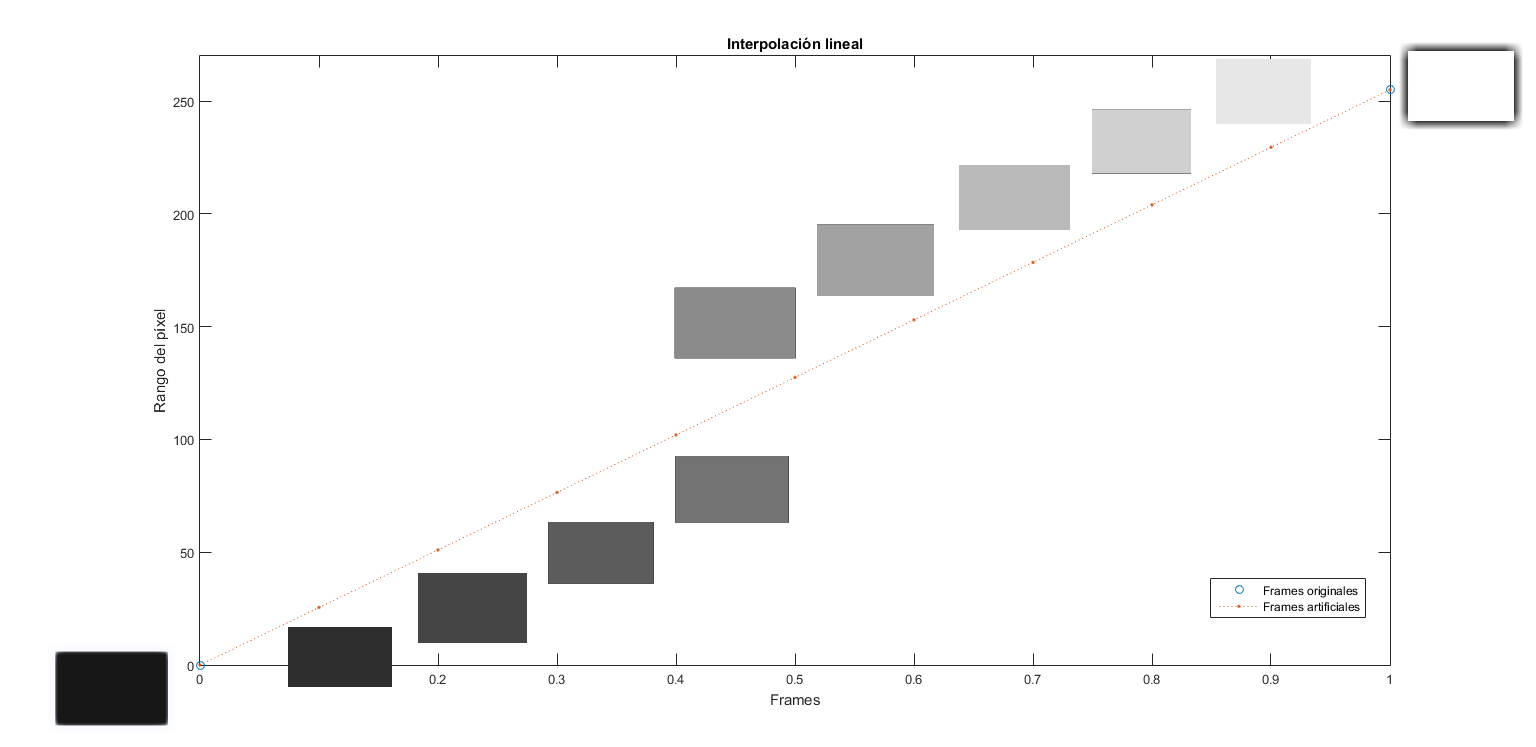
\includegraphics[width=0.75\textwidth]{GraficoLineal.png}
     \caption{Muestra del momento en que se realiza el cambio de negro a blanco, con sus respectivos frames intermedios}\label{fig:linealValidacion}
\end{figure}
\noindent

\subsubsection*{\bf{Splines}}

Seguimos con la misma metodolog\'ia que con interpolaci\'on lineal, definiendo la funci\'on en cuesti\'on:

$$f(x) = a + b (x - x_0) + c (x - x_0)^2 + d (x - x_0)^3$$

Pero ¿c\'omo hallamos los coeficientes del polinomio? Podr\'iamos realizar las cuentas en papel y seguir con el procedimiento de verificar con respecto a la implementaci\'on. Sin embargo, ser\'ia bastante engorroso de realizar, por lo que optamos por usar \emph{MatLab}. Usando la funci\'on $interpo1$ podemos obtener el valor de cualquier punto intermedio, en particular los que se evaluaron en nuestro programa.

No obstante, si bien notamos que en este caso particular la funci\'on $f(x)$ debería asemejarse a una funci\'on lineal (una instancia particular de un polinomio cúbico), hay que tener en cuenta una característica de \emph{Splines}: la construcci\'on por bloques. Como decidimos que cada bloque comparta su primer y \'ultimo frame (excepto los extremos, que comparten alguno de los 2) no existe el caso en que se divida de forma discontinua.

Ideamos una instancia con cantidad de frames a adicionar igual 5, dividido en 16 bloques. Dicho esto, mediante \emph{MatLab} visualizamos cada Spline generado por bloque.

\subsubsection*{Resultado}

Comparando con la implementaci\'on no se encontr\'o ninguna diferencia con lo ya comentado.

En el gr\'afico \ref{fig:splineValidacion} observamos lo que \emph{MatLab} produjo al enviarle los puntos pertenecientes al bloque donde se hallaba el cambio de negro a blanco. Comparando con los frames que obtuvimos, la similitud es evidente.

\begin{figure}[h!]
  \centering
    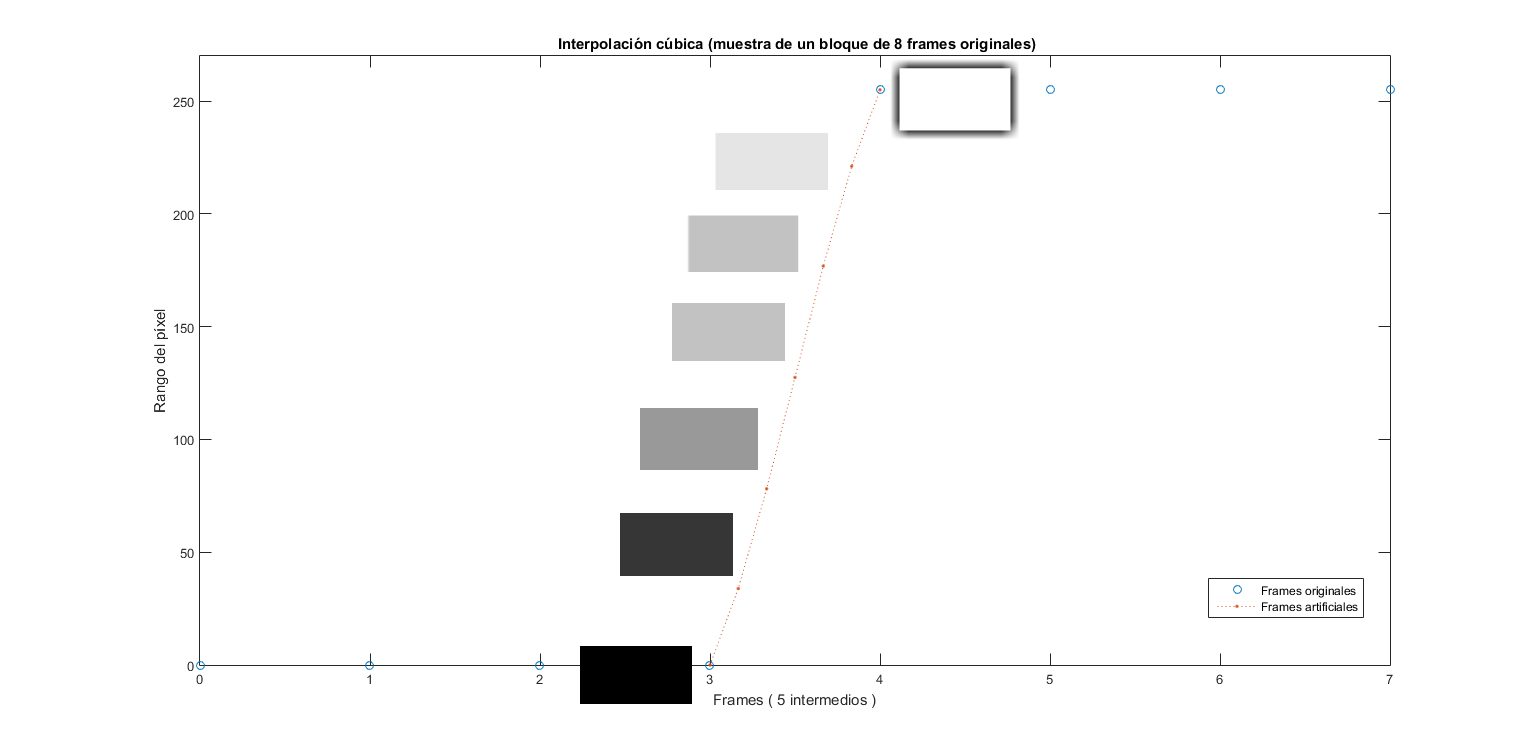
\includegraphics[width=0.75\textwidth]{GraficoSplines.png}
     \caption{Muestra del bloque que contiene el cambio, con los cuadros comparados}\label{fig:splineValidacion}
\end{figure}
\noindent

%---------------------------------------------------------------
\subsubsection{C\'amara Fija - Im\'agen Fija}

Este experimento es equivalente a considerar una im\'agen estática reproducida durante un lapso de tiempo. Difiere con el hecho de una c\'amara filmando un objeto inmóvil pues esta filmación puede tener alteraciones producidas por las diferencias de luz en cada instante capturado por la cámara. Y est\'a claro que el mero hecho de querer ralentizar un video de tal caracter\'istica solo servir\'a para aumentar la duraci\'on de la misma. Si la implementaci\'on se realiz\'o de forma correcta, no debería existir ning\'un cambio en el video.

Usamos metodolog\'ias id\'enticas para los tres m\'etodos. Esto es, extraer cada cuadro artificial y corroborar que coincide con la foto utilizada.

\subsubsection*{Resultado}

Obviamente, Vecino más cercano se comportó de la forma esperada. Pero también lo hicieron los otros dos métodos: como en cada p\'ixel $(i,j)$ el valor se mantuvo constante, las funciones interpoladoras se convirtieron en funciones constantes (polinomios de grado 0). De esta manera, más frames a generar solo producían un video idéntico pero más largo. La im\'agen permenece intacta durante toda la reproducci\'on.
